\documentclass[a4paper]{article}

\usepackage{amsmath}
\usepackage{tabularx}
\usepackage{todonotes}
%\usepackage{showframe}
\usepackage{ upgreek }
\usepackage{tikz}
\newcommand{\specialcell}[2][c]{%
  \begin{tabular}[#1]{@{}c@{}}#2\end{tabular}}

\begin{document}
\section{Organization and Introduction}
\begin{itemize}
\item The Art of managing complexity
\begin{itemize}
\item Abstraction: Hiding details when they are not important
\item Discipline: Intentionally restricting your design choices so that you can work more productively at higher abstraction levels
\item The three -Y's
\begin{itemize}
\item Hierarchy: A system is divided into modules of smaller complexity
\item Modularity: Having well defined functions and interfaces
\item Regularity: Encouraging uniformity, so modules can be easily re-used
\end{itemize}
\end{itemize}
\item Bit: \textbf{B}inary dig\textbf{it}
\end{itemize}

\section{Binary Numbers}
\begin{itemize}
\item Powers of two:\\
\begin{tabular}{c|c|c}
$2^0= 1$ & $2^5=32$ & $2^{10}= 1024$\\ 
$2^1= 2$ & $2^6=64$ & $2^{11}= 2048$\\ 
$2^2= 4$ & $2^7=128$ & $2^{12}= 4096$\\ 
$2^3= 8$ & $2^8=256$ & $2^{13}= 8192$\\ 
$2^4= 16$ & $2^9=512$ & $2^{14}= 16384$\\ 
\end{tabular}
\item Binary to decimal conversion
\begin{align*}
10011_2&=2^4\times 1 +2^3\times 0 + 2^2\times 0 +2^1\times 1 +2^0\times 1\\
&=16 \times 1+8 \times 0+4 \times 0+2 \times 1+1 \times 1\\
&=16+0+0+2+1=19_{10}
\end{align*}
\item Convert decimal to binary (roughly). Example with $47_{10}$ to binary\\
\begin{tabular}{c|c|c|c|c}
$2^6=64$& is $64\leq 47$?&no&0&do nothing\\ 
$2^5=32$& is $32\leq 47$?&yes&1&47-32=15\\
$2^4=16$& is $16\leq 15$?&no&0&do nothing\\
$2^3=8$& is $8\leq 15$?&yes&1&15-8=7\\ 
$2^2=4$& is $4\leq 7$?&yes&1&7-4=3\\
$2^1=2$& is $2\leq 3$?&yes&1&3-2=1\\
$2^0=1$& is $1\leq 1$?&yes&1&1-1=0; done!\\
\end{tabular}\\
$\Rightarrow 47_{10}$ to binary is $0101111_2$ 
\item Binary values and range
\begin{itemize}
\item $N-$digit decimal number
\begin{itemize}
\item How many values: $10^N$
\item Range: $\lbrack 0,10^{N}-1\rbrack$
\item Example (3-digit number): $10^3=1000$ possible values, range:$\lbrack 0,999\rbrack$
\end{itemize}
\item $N-$bit binary number
\begin{itemize}
\item How many values: $2^N$
\item Range: $\lbrack 0,2^{N}-1\rbrack$
\item Example (3-digit number): $2^3=8$ possible values, range:$\lbrack 0,7\rbrack=\lbrack 000_2\text{ to }111_2\rbrack$
\end{itemize}
\end{itemize}
\item Hexadecimal (Base-16) Numbers\\
\begin{tabular}{c|c|c|c|c|c|c}
Decimal & Hexadecimal & Binary&{}&Decimal & Hexadecimal & Binary\\\hline
0&0&0000&{}&8&8&1000\\
1&1&0001&{}&9&9&1001\\
2&2&0010&{}&10&A&1010\\
3&3&0011&{}&11&B&1011\\
4&4&0100&{}&12&C&1100\\
5&5&0101&{}&13&D&1101\\
6&6&0110&{}&14&E&1110\\
7&7&0111&{}&15&F&1111\\
\end{tabular}
\item Bits, Bytes, Nibbles...
\[\begin{array}{*{20}{c}}
{\underbrace 1_{{\text{MSB}}}001011\underbrace 0_{{\text{LSB}}}}&{\overbrace {1001\underbrace {0110}_{{\text{nibble}}}}^{{\text{Byte}}}}&{\underbrace {{\text{CE}}}_{{\text{MSB}}}{\text{BF9A}}\underbrace {{\text{D7}}}_{{\text{LSB}}}}
\end{array}\]
Where MSB=Most significant Bit and LSB=Least significant Bit
\item Addition in base two works exactly the same as in base 10, using carries
\item Overflow
\begin{itemize}
\item Digital systems operate on a fixed number of bits
\item Addition overflows when the result is too big to fit in the available number of bits
\end{itemize}
\item Signed Binary Numbers
\begin{itemize}
\item Sign/Magnitude Numbers
\begin{itemize}
\item 1 sign bit, $N-1$ magnitude bits
\item Sign bit is the most significant (left-most) bit
\item Example: 4-bit sign/mag repr. of $\pm 6$:
\begin{itemize}
\item $+6=\textbf{0}110$
\item $-6=\textbf{1}110$
\end{itemize}
\item Range of an $N-$bit sign/magnitude number:\\
$\lbrack -\left( 2^{N-1}-1\right),2^{N-1}-1\rbrack$
\item Problems:
\begin{itemize}
\item Addition doesn't work
\item Two representations of 0 ($\pm 0$): 1000 and 0000
\item Introduces complexity in the processor design
\end{itemize}
\end{itemize}
\item One's Complement Numbers
\begin{itemize}
\item A negative number is formed by reversing the bits of the positive number (MSB still indicates the sign of the integer)\\
\begin{tabular}{|c|c|c|c|c|c|c|c|c|c|c|}
\hline
$2^7$&$2^6$&$2^5$&$2^4$&$2^3$&$2^2$&$2^1$&$2^0$&{}&One's Compl.&Unsigned\\\hline\hline
0&0&0&0&0&0&0&0&$=$&0&0\\
0&0&0&0&0&0&0&1&$=$&1&1\\
0&0&0&0&0&0&1&0&$=$&2&2\\
\dots&\dots&\dots&\dots&\dots&\dots&\dots&\dots&\dots&\dots&\dots\\
0&1&1&1&1&1&1&1&$=$&127&127\\
1&0&0&0&0&0&0&0&$=$&-127&128\\
1&0&0&0&0&0&0&1&$=$&-126&129\\
\dots&\dots&\dots&\dots&\dots&\dots&\dots&\dots&\dots&\dots&\dots\\
1&1&1&1&1&1&0&1&$=$&-2&253\\
1&1&1&1&1&1&1&0&$=$&-1&254\\
1&1&1&1&1&1&1&1&$=$&-0&255\\\hline
\end{tabular}
\item Range of $n-$bit number: $\lbrack -2^{n-1}-1,2^{n-1}-1\rbrack$, 8 bits:$\lbrack -127,127\rbrack$
\item Addition: Done using binary addition with end-around carry. If there is a carry out of the MSB of the sum, this bit must be added to the LSB of the sum
\end{itemize}
\item Two's Complement Numbers
\begin{itemize}
\item Don't have same problems as sign/magnitude numbers:
\begin{itemize}
\item addition works
\item Single representation for 0
\end{itemize}
\item Has advantages over one's complement:
\begin{itemize}
\item Has a single 0 representation
\item Eliminates the end-around carry operation required in one's complement addition.
\end{itemize}

\item A negative number is formed by reversing the bits of the positive number (MSB still indicates the sign of the integer) and adding 1:\\
\begin{tabular}{|c|c|c|c|c|c|c|c|c|c|c|}
\hline
$2^7$&$2^6$&$2^5$&$2^4$&$2^3$&$2^2$&$2^1$&$2^0$&{}&Two's Compl.&Unsigned\\\hline\hline
0&0&0&0&0&0&0&0&$=$&0&0\\
0&0&0&0&0&0&0&1&$=$&1&1\\
0&0&0&0&0&0&1&0&$=$&2&2\\
\dots&\dots&\dots&\dots&\dots&\dots&\dots&\dots&\dots&\dots&\dots\\
0&1&1&1&1&1&1&1&$=$&127&127\\
1&0&0&0&0&0&0&0&$=$&-128&128\\
1&0&0&0&0&0&0&1&$=$&-127&129\\
\dots&\dots&\dots&\dots&\dots&\dots&\dots&\dots&\dots&\dots&\dots\\
1&1&1&1&1&1&0&1&$=$&-3&253\\
1&1&1&1&1&1&1&0&$=$&-2&254\\
1&1&1&1&1&1&1&1&$=$&-1&255\\\hline
\end{tabular}
\item Same as unsigned binary, but the most significant bit (MSB) has value of $-2^{N-1}$
\begin{itemize}
\item Most positive 4-bit number: 0111
\item Most negative 4-bit number: 1000
\end{itemize}
\item The most significant bit still indicates the sign (1=neg., 0=pos.)
\item Range of an $N-$bit two's comp. number: $\lbrack -2^{N-1},2^{N-1}-1\rbrack$, 8 bits:$\lbrack -128,127\rbrack$
\end{itemize}
\end{itemize}
\item Increasing bit width (assume from $N$ to $M$, with $M>N$): 
\begin{itemize}
\item Sign-extension
\begin{itemize}
\item Sign bit is copied into MSB
\item Number value remains the same
\item Give correct result for two's compl. numbers
\item Example 1:
\begin{itemize}
\item 4-bit representation of $3=\textbf{0}011$
\item 8-bit sign-extended value: $\textbf{00000}011$
\end{itemize}
\item Example 2:
\begin{itemize}
\item 4-bit representation of $-5=\textbf{1}011$
\item 8-bit sign-extended value: $\textbf{11111}011$
\end{itemize}
\end{itemize}
\item Zero-extension
\begin{itemize}
\item Zeros are copied into MSB
\item Value will change for negative numbers
\item Example 1:
\begin{itemize}
\item 4-bit value: $0011_2=3_{10}$
\item 8-bit zero-extended value: $\textbf{0000}0011_2=3_{10}$
\end{itemize}
\item Example 2:
\begin{itemize}
\item 4-bit value: $1011_2=-5_{10}$
\item 8-bit zero-extended value: $\textbf{0000}1011_2=\textbf{$11_{\textbf{10}}$}$
\end{itemize}
\end{itemize}
\end{itemize}
\end{itemize}

\section{Short Introduction to Electrical Engineering (EE Perspective)}
\begin{itemize}
\item The goal of circuit design is to optimize:
\begin{itemize}
\item Area: Net circuit area is proportional to the cost of the device
\item Speed/Throughput: We want circuits that work  faster, or do more
\item Power/Energy
\begin{itemize}
\item Mobile devices need to work with a limited power supply
\item High performance devices dissipate more than 100W/$cm^2$
\end{itemize}
\item Design time
\begin{itemize}
\item Designers are expensive
\item The competition will not wait for you
\end{itemize}
\end{itemize}
\item (Frank's) Principles for engineering
\begin{itemize}
\item Good engineers are lazy: They do not want to work unnecessarily, be creative
\item They know how to ask the question ``why''?: take nothing for granted
\item Engineering is not a religion: Use what works best for you
\item Keep it simple and stupid: Engineers' job is to manage complexity
\end{itemize}
\item Building blocks for microchips
\begin{itemize}
\item Conductors: Metals (Aluminium, Copper)
\item Insulators: Glass (SiO$_2$), Air
\item Semiconductors: Silicon (Si), Germanium (Ge)
\end{itemize}
\item N-type Doping: Add extra electron (negatively charged), zone becomes negatively charged\todo{Maybe add a definition or a better explanation}
\item P-type Doping: Remove electron, zone becomes positively charged
\item Semiconductors:
\begin{itemize}
\item You can ``Engineer'' its properties, i.e.
\begin{itemize}
\item Make it P type by injecting type-III elements (b, Ga, In)
\item Make it N type by injecting elements from type-V (P, As)
\end{itemize}
\item You can combine P and N regions to each other, from a pure semiconductor
\item Allows you to make interesting electrical devices (Diodes, Transistors, Thrystors)
\end{itemize}
\item pMOS is a P type transistor, nMOS an N type transistors; combined they are a CMOS
\item CMOS (Properties)
\begin{itemize}
\item No input current: Capacitive input, no resistive path from the input
\item No current when output is at logic levels: Little static power, current is needed only when switching
\item Electrical properties determined directly by geometry: A transistor that is 2 times larger drives twice the current
\item Very simple to manufacture: pMOS and nMOS can be manufactures on the same substrate
\end{itemize}
\item CMOS Gate Structure
\begin{itemize}
\item The general form used to construct any inverting logic, such as: NOT, NAND, NOR
\begin{itemize}
\item The networks may consist of transistors in series or parallel
\item When transistors are in parallel, the network is ON if either transistor is ON
\item When transistors are in series, the network is ON only if all transistors are ON
\end{itemize}
\item In a proper logic gate: One of the networks should be ON and the other OFF at any given time
\item Use the rule of conduction complements:
\begin{itemize}
\item When nMOS transistors are in series, the pMOS transistor must be in parallel
\item When nMOS transistors are in parallel, the pMOS transistors must be in series
\end{itemize}
\end{itemize}
\todo[inline]{Add picture on slide 34, 03 - EEPerspective}
\item Logic Gates
\begin{itemize}
\item Perform logic functions: Inversion (NOT), AND, OR, NAND, NOR, etc.
\item Single input: NOT gate, buffer
\item Two-input: AND, OR, XOR, NAND, NOR, XNOR\\
\includegraphics[scale=0.27]{Figures/commonLogicGates.jpg}
\item Multiple-Input:
\begin{itemize}
\item 3, 4, or even more input AND, OR, XOR gates
\item Compound gates
\begin{itemize}
\item AND-OR
\item OR-AND
\item AND-OR-INVERT
\item OR-AND-INVERT
\end{itemize}
\item Other cells: Multiplexers and Adders
\end{itemize}
\end{itemize}
\item Logic Levels
\begin{itemize}
\item Define ranges of discrete voltages to represent 1 and 0 (i.e. 0 for ground and 1 for 5V ($V_{DD}$)) and allow for noise.
\end{itemize}
\item Noise: Is anything that degrades the signal (i.e. resistance, power supply noise, etc.)
\item Moore's Law
\begin{itemize}
\item \emph{``Number of transistors that can be manufactured doubles roughly every 18 months.''} - Gordon Moore, 1965
\end{itemize}
\item How do we keep Moore's Law:
\begin{itemize}
\item Manufacturing smaller structures: some structures are already a few atoms in size
\item Developing materials with better properties
\item Optimizing the manufacturing steps
\item New technologies
\end{itemize}
\item Power consumption
\begin{itemize}
\item Power = Energy consumed per unit time
\item Two types of power consumption:
\begin{enumerate}
\item Dynamic power consumption: Power to charge transistor gate capacitances \[P_{\text{dynamic}}=\frac{1}{2}CV_{DD}^2f\]
\item Static power consumption: Power consumed when no gates are switching, caused by the leakage current \[P_{\text{static}}=I_{DD}V_{DD}\]
\end{enumerate}
\end{itemize}
\item Power Consumption example:
\begin{itemize}
\item Estimate the power consumption of a wireless handheld computer
\begin{itemize}
\item $V_{DD}=1.2V$
\item $C=20nF$
\item $f=1 GHz$
\item $I_{DD}=20 mA$
\begin{align*}
P_{\text{total}}&=P_{\text{dynamic}}+P_{\text{static}}\\
&=\frac{1}{2}CV_{DD}^2f+I_{DD}V_{DD}\\
&=\frac{1}{2}(20 nF)(1.2V)^2(1GHz)+(20mA)(1.2V)\\
&=14.4 W
\end{align*}
\end{itemize}
\end{itemize}

\end{itemize}

\section{Combinational Circuits: Theory}
\begin{itemize}
\item Circuit elements. A circuit consists of:
\begin{itemize}
\item Inputs
\item Outputs
\item Nodes (wires): Connections between I/O and circuit elements. To count them, look at
\begin{itemize}
\item Outputs of every circuit elements
\item Inputs to the entire circuit
\end{itemize}
\item Circuit elements
\end{itemize}
\item Types of Logic Circuits
\begin{itemize}
\item Combinational Logic
\begin{itemize}
\item Memoryless
\item Outputs determined by current values of inputs
\item In some books called Combinatorial Logic
\end{itemize}
\item Sequential Logic
\begin{itemize}
\item Has Memory
\item Outputs determined by previous and current values of inputs
\end{itemize}
\end{itemize}
\item Rules of Combinational Composition
\begin{itemize}
\item Every circuit element is itself combinational
\item Every node of the circuit is either
\begin{itemize}
\item Designated as an input to the circuit
\item Connects to exactly one output terminal of a circuit element
\end{itemize}
\item The circuit contains no cyclic paths: Every path through the circuit visits each node at most once

\end{itemize}
\item Boolean Equations\footnote{For a more in depth look, use the material from Diskrete Mathematik}
\begin{itemize}
\item Functional specifications of outputs in terms of inputs.
\end{itemize}
\item Boolean Algebra
\begin{itemize}
\item Set of axioms and theorems to simplify Boolean equations
\item Like regular algebra, but in some cases simpler because variables only have 1 or 0 as a value
\item Axioms and theorems obey the principles of duality:
\begin{itemize}
\item Stay corrected if: ANDs and ORs interchanged and 0's and 1's interchanged
\item Example:\\
\begin{tabular}{l|l}
{}&Dual\\\hline
$\overline{0}=1$&$\overline{1}=0$\\
$B\cdot\overline{B}=0$&$B+\overline{B}=1$
\end{tabular}

\end{itemize}
\end{itemize}
\item Boolean Axioms\\
\begin{tabular}{|l|l|l|l|l|}\hline
{}&Axiom&{}&Dual&Name\\\hline
$A1$ & $B=0$ if $B\not = 1$ & $A1'$ & $B=1$ if $B\not=0$ & Binary Field\\
$A2$ & $\overline{0}=1$ & $A2'$ & $\overline{1}=0$ & NOT  \\
$A3$ & $0\cdot 0=0$ & $A3'$ & $1+1=1$ & AND/OR     \\
$A4$ & $1\cdot 1=1$ & $A4'$ & $0+0=0$ & AND/OR    \\
$A5$ & $0\cdot 1=1\cdot 0=0$ & $A5'$ & $1+0=0+1=1$ & AND/OR \\ \hline
\end{tabular}
\\Duality: If the symbols 0 and 1 and the operators $\cdot$ (AND) and $+$ (OR) are interchanged, the statement will still be correct
\item Boolean Theorems\\
\resizebox{13cm}{!}{
\begin{tabular}{|l|l|l|l|l|}\hline
{}&Theorem&{}&Dual&Name\\\hline\hline
$T1$ & $B\cdot 1=B$ & $T1'$ & $B+0=B$ & Identity\\\hline
$T2$ & $B\cdot 0=0$ & $T2'$ & $\overline{1}=0$ & Null Element  \\\hline
$T3$ & $B\cdot B=B$ & $T3'$ & $1+1=1$ & Idempotency     \\\hline
$T4$ & {} & $\overline{\overline{B}}=B$ & {} & Involution    \\\hline
$T5$ & $B\cdot\overline{B}=0$ & $T5'$ & $1+0=0+1=1$ & Complements \\ \hline
$T6$ & $B\cdot C=C\cdot B$ & $T6'$ & $B+C=C+B$ & Commutativity	\\\hline
$T7$ & $(B\cdot C)\cdot D= B\cdot (C\cdot D)$ & $T7'$ & $(B+C)+D = B+(C+D)$ & Associtivity	\\\hline
$T8$ & $(B\cdot C)+(B\cdot D)=B\cdot (C+D)$ & $T8'$ & $(B+C)\cdot (B+D)=B+(C\cdot D)$ & Distributivity	\\\hline
$T9$ & $B\cdot (B+C)=B$ & $T9'$ & $B+(B\cdot C)=B$ & Covering	\\\hline
$T10$ & $(B\cdot C) + (B\cdot \overline{C})=B$ &$T10'$& $(B+C)\cdot (B+\overline{C})=B$& Combining\\\hline
$T11$ &\specialcell{$(B\cdot C)+(\overline{B}\cdot D)+(C\cdot D)$\\$=B\cdot C+\overline{B}\cdot D$} & $T11'$ & \specialcell{$(B+t C)\cdot(\overline{B}+ D)\cdot(C+ D)$\\$=(B + C)\cdot(\overline{B}+ D)$}  & Consensus	\\\hline
$T12$ & $\overline{B_0\cdot B_1\cdot B_2\cdot\dots}= (\overline{B_0}+\overline{B_1}+\overline{B_2}+\dots)$ & $T12'$ & $\overline{B_0 +  B_1+ B_2+\dots}= (\overline{B_0}\cdot\overline{B_1}\cdot\overline{B_2}\cdot\dots)$ & \specialcell{De Morgan's\\ Theorem}\\
\hline
\end{tabular}
}

\item Bubble Pushing
\begin{itemize}
\item Pushing bubbles backward (from the output) or forward (from the inputs) changes the body of the gate from AND to OR or vice versa
\begin{itemize}
\item Pushing a bubble from the output back to the inputs puts bubbles on all gate inputs
\item Pushing bubbles on all gate inputs forward toward the output puts a bubble on the output and changes the gate body
\includegraphics[scale=0.35]{Figures/bubblePushing.jpg}
\end{itemize}
\item Rules:
\begin{itemize}
\item Begin at the output of the circuit and work toward the inputs
\item Push any bubbles on the final output back toward the inputs
\item Draw each gate in a form so that bubbles cancel
\end{itemize}
\end{itemize}
\end{itemize}

\section{Combinational Circuits Design}
\begin{itemize}
\item Some Definitions:
\begin{itemize}
\item Complement: variable with a bar over it ($\overline{A},\overline{B},\overline{C}$)
\item Literal: variable or its complement ($A,\overline{A},B,\overline{B},C,\overline{C}$)
\item Implicant: product (AND) of literals ($A\cdot B\cdot \overline{C}$)
\item Minterm: product (AND) that includes all input variables ($A\cdot B \cdot \overline{C}$)
\item Maxterm: sum (OR) that includes all input variables ($A+\overline{B}+\overline{C}$)
\end{itemize}
\item Sum-of-Products (SOP) Form
\todo[inline]{aggiungere tabella cerchiata ai valori Y=1}
\begin{center}
\begin{tabular}{c c|c|c}
A&B&Y&minterm\\\hline
0&0&0&$\overline{A}\overline{B}$\\
0&1&1&$\overline{A}B$\\
1&0&0&$A\overline{B}$\\
1&1&1&$AB$
\end{tabular}
$$Y=F(A,B)=(\overline{A}\cdot B)+(A\cdot B)$$
\end{center}
\begin{itemize}
\item All boolean equations can be written in SOP form
\begin{itemize}
\item Each row in a truth table has a minterm
\item A minterm is a product (AND) of literals
\item Each minterm is TRUE for that row (and only that row)
\end{itemize}
\item Formed by ORing the minterms for which the output is TRUE
\end{itemize}
\item The Dual: Product-of-Sums (POS) Form
\todo[inline]{aggiungere tabella cechiata ai valori Y=0}
\begin{center}
\begin{tabular}{c c|c|c}
A&B&Y&maxterm\\\hline
0&0&0&$A+B$\\
0&1&1&$A+\overline{B}$\\
1&0&0&$\overline{A}+B$\\
1&1&1&$\overline{A}+\overline{B}$
\end{tabular}
$$Y=F(A,B)=(A+B)\cdot (\overline{A}+B)$$
\end{center}
\begin{itemize}
\item All Boolean equations can be written in POS form
\begin{itemize}
\item Each row in a truth table has a maxterm
\item A minterm is a sum (OR) of literals
\item Each minterm is FALSE for that row (and only that row)
\end{itemize}
\item Formed by ANDing the maxterms for which the output is FALSE
\end{itemize}
\item Karnaugh Maps (K-Maps)
\begin{itemize}
\item Boolean expressions can be minimized by combining terms
\item K-maps minimize equations graphically
\item Rules:
\begin{itemize}
\item Special order for bit combinations: $\mathop {00,01,11,10}\limits^{
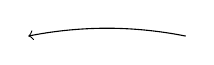
\begin{tikzpicture}
\draw[<-] (0,0) parabola bend (1,0.1) (2,0);
\end{tikzpicture}
}$ (only one bit changes to the next)
\item Every 1 in a K-map must be circled at least once
\item Each circle must span a power of 2 ($2^0$ included) squares in each direction 
\item Each circle must be as large as possible
\item A circle may wrap around the edges of the K-map
\item A ``Don't care'' $(X)$ is circled only if it helps minimize the equation
\end{itemize}
\end{itemize}
\item Circuit schematics 
\begin{itemize}
\item Inputs: left (or top) side of a schematic
\item Outputs: right (or bottom) side of a schematic
\item Circuits should flow from left to right
\item Straight wires are better than wires with multiple corners
\item Wires always connect at a T junction
\item A dot where wires cross indicated a connection between the wires
\item Wires crossing without a dot make no connection
\end{itemize}
\item Additional Logic Levels: $X$ and $Z$
\begin{itemize}
\item Contention: $X$
\begin{itemize}
\item When a signal is being driven to 1 and 0 simultaneously
\item Not a real level, could be any value (1,0 or something in between)
\item Usually a problem:
\begin{itemize}
\item Two outputs drive one node to opposite values
\item Normally there should only be one driver for every connection
\end{itemize}
\item WARNING: ``Don't care'' and ``contention'' are both called $X$
\begin{itemize}
\item These are not the same
\item Verilog uses $X$ for both, VHDL uses ``-'' for don't care, and ``$X$'' for contention
\item Don't care: degree of freedom that is fixed at implementation time
\item Contention: a bug really, undetermined behaviour
\end{itemize}
\end{itemize}
\item High-impedance or tri-state (or Floating): $Z$
\begin{itemize}
\item When an output is not driving to any specific value
\item Means the output is disconnected
\item Not a real level, some other output is able to determine the level
\item Output is called Floating, high impedance, tri-stated, or high-$Z$
\item Floating output might be 0, 1 or somewhere in between
\item Floating nodes are used in tri-state busses:
\begin{itemize}
\item Many different drivers share one common connection
\item Exactly one driver is active at any time
\item All the other drivers are ``disconnected''
\item The disconnected drivers are said to be floating, allowing exactly one node to drive
\item More than one input can listen to the shared bus without problems
\end{itemize}
\end{itemize}
\end{itemize}
\item Combinational Building Blocks
\begin{itemize}
\item Combinational logic is often grouped into larger building blocks to build more complex systems
\item Hide the unnecessary gate-level details to emphasize the function of the building block (full adders, priority circuits, etc.)
\end{itemize}
\item Multiplexer (Mux)
\begin{itemize}
\item Selects between one of $N$ inputs to connect to the output
\item Needs $\log_2N-$bit control input
\item A 4:1 Multiplexer can be implemented with:
\begin{itemize}
\item Two-level logic
\item Tristate buffers
\item Tree of 2:1 muxes
\end{itemize}
\item In general, a $2^N-$input multiplexer can be programmed to perform any $N-$input logic function by applying 0's and 1's to the appropriate data inputs
\end{itemize}
\item Decoders
\begin{itemize}
\item $N$ inputs, $2^N$ outputs
\item One-hot outputs: only one output HIGH at once
\end{itemize}
\item Timing
\begin{itemize}
\item Propagation delay: $t_{pd}=$ max delay from input to output
\item Contamination delay: $t_{cd}=$ min delay from input to output\\
\includegraphics[scale=0.3]{Figures/PropContDelay.jpg}
\item Delay is caused by 
\begin{itemize}
\item capacitance and resistance in a circuit
\item Speed of light limitation (not as fast as you think)
\end{itemize}
\item Reasons why $t_{pd}$ and $t_{cd}$ may be different:
\begin{itemize}
\item Different rising and falling delays
\item Multiple inputs and outputs, some of which are faster than other
\item Circuits slow down when hot and speed up when cold
\end{itemize}
\item Critical (Long) and short paths\\
\includegraphics[scale=0.25]{Figures/CriticalAndShortPath.jpg}
\begin{itemize}
\item Critical (Long) path: $t_{pd}=2t_{pd\_\text{AND}}+t_{pd\_\text{OR}}$
\item Short path: $t_{cd}=t_{cd\_\text{AND}}$
\end{itemize}
\item Propagation Times\\
\begin{tabular}{l|l}
Gate & $t_{pd}$(ps)\\\hline
NOT & 30\\
$2-$input AND & 60\\
$3-$input AND & 80\\
$4-$input OR & 90\\
tristate ($A$ to $Y$) & 50\\
tristate (enable to $Y$) & 35
\end{tabular}
\end{itemize}
\item Glitches
\begin{itemize}
\item Glitch: when a single input change causes multiple output changes
\item Glitches don't cause problems because of synchronous design conventions
\item But it's important to recognize a glitch when you see one in timing diagrams
\item In general a glitch can occur when a change in a single variable crosses the boundary between two prime implicants in a $K-$map.
\item You \textbf{can't} get rid of all glitches - simultaneous transitions on multiple inputs can also cause glitches
\end{itemize}
\end{itemize}

\section{Field Programmable Gate Array (FPGA)}
\begin{itemize}
\item Logic arrays
\begin{itemize}
\item Programmable logic arrays (PLAs)
\begin{itemize}
\item AND array followed by OR array
\item Perform combinational logic only
\item Fixed internal connections
\item Composed of:
\begin{itemize}
\item LUTs (LookUp Tables): perform combinational logic
\item Flip-flops: perform sequential functions
\item Multiplexers connect LUTs and flip-flops
\end{itemize}
\end{itemize}
\item Field programmable gate arrays (FPGAs)
\begin{itemize}
\item Array of configurable logic blocks (CLBs)
\item Perform combinational and sequential logic
\item Programmable internal connections
\item Composed of:
\begin{itemize}
\item CLBs (Configurable Logic Blocks): Perform logic
\todo[inline]{too deeply nested}
\item \textbf{LUT}s (\textbf{L}ook\textbf{U}p \textbf{T}ables): perform combinational logic
\item Flip-flops: performs sequential functions
\item Multiplexers: connect LUTs and flip-flops
\todo[inline]{fino qua}
\item IOBs (Input/Output Buffers): Interface with outside world
\item Programmable interconnection: connect CLBs and IOBs
\end{itemize}
\item Some FPGAs include other building blocks such as multipliers and RAMs
\end{itemize}
\end{itemize}
\end{itemize}


\section{Verilog for Combinational Circuits}
\begin{itemize}
\item Two hardware description languages
\begin{itemize}
\item Verilog
\begin{itemize}
\item Developed in 1984
\item Became an IEEE standard (1364) in 1995
\item More popular in US
\end{itemize}
\item VHDL
\begin{itemize}
\item Developed in 1981
\item Became an IEEE standard (1076) in 1987
\item More popular in Europe
\end{itemize}
We used Verilog
\end{itemize}
\item Defining a module
\begin{itemize}
\item A module is the main buliding block in Verilog
\item Need to declare:
\begin{itemize}
\item Name of the module
\item Types of its connections (input, output)
\item Names of its connections
\end{itemize}
\end{itemize}
\textit{The following two codes are identical}\\
\includegraphics[scale=0.25]{Figures/DefiningModuleExample2ways.jpg}
\item You can also define multi-bit busses
\begin{itemize}
\item \lbrack \texttt{range\_start : range\_end}\rbrack
\end{itemize}
\textit{Example}\\
\includegraphics[scale=0.25]{Figures/BussesExample.jpg}
\item Basic Syntax
\begin{itemize}
\item Verilog is case sensitive:
\begin{itemize}
\item SomeName \textbf{and} somename \textbf{are not the same!}
\end{itemize}
\item Names cannot start with numbers:
\begin{itemize}
\item 2good \textbf{is not a valid name}
\end{itemize}
\item White space is ignored
\item Comments
\begin{itemize}
\item Single Line comment starts with //
\item Multiline comments start and end with /*...*/ 
\end{itemize}
Remember:
\begin{itemize}
\item Use a consistent naming style
\item Use MSB to LSB ordering for busses, e.g a\lbrack31:0\rbrack and not a\lbrack0:31\rbrack
\item Define one module per file, it makes managing your design hierarchy easier
\item Use a file name that equals your module name
\end{itemize}
\end{itemize}
\item Two main HDL's styles
	\begin{itemize}
		\item Structural
			\begin{itemize}
				\item Describe how modules are interconnected
				\item Each module contains other modules (instances) and interconnections between them
				\item Describes a hierarchy
			\end{itemize}
		\item Behavioral
			\begin{itemize}
				\item The module body contains functional description of the circuit
				\item Contains logical and mathematical operators	
			\end{itemize}
	\end{itemize}
\todo[inline]{quando togli il todo, il titolo dell'immagine e l'immagine vengono separati su due pagine}
	\textit{Structural HDL Example}\\
		\includegraphics[scale=0.3]{Figures/StructuralHDLExample.jpg}
\item Behavioral HDL: Defining Functionality\\
	\includegraphics[scale=0.26]{Figures/BehavioralHDL_DefiningFunctionality.jpg}
\item Bitwise Operators\\
	\includegraphics[scale=0.30]{Figures/BitwiseOperators.jpg}
\item Reduction Operators\\
	\includegraphics[scale=0.30]{Figures/ReductionOperators.jpg}
\item Conditional Assignments\\
	\includegraphics[scale=0.25]{Figures/ConditionalAssignments.jpg}
\item How to express numbers
	\center{\huge{\color{red}N\color{black}'\color{blue}B\color{green}xx}}
	\center{\Large{\color{red}8\color{black}'\color{blue}b\color{green}0000\_0001}}
	\begin{itemize}
		\item \color{red}(N) Number of bits\color{black}
			\begin{itemize}
				\item Expresses how many bits will be used to store the value
			\end{itemize}
		\item \color{blue}(B) Base\color{black}
			\begin{itemize}
				\item Can be n (binary), h (hexadecimal), d (decimal), o (octal)
			\end{itemize}
		\item \color{green}(xx) Number\color{black}
			\begin{itemize}
				\item The value expressed in base, aparto from numbers it can also have X and Z as values
				\item Underscore\_ can be used to improve readability
			\end{itemize}	
	\end{itemize}
	\end{itemize}
\begin{itemize}
\item Number representation in Verilog\\
	\begin{tabular}{l|l}
	Verilog&Stored Number\\\hline
	$4'b1001$&$1001$\\
	$8'b1001$&$0000\enspace1001$\\
	$8'b0000\_1001$&$000\enspace1001$\\
	$8'bxX0X1zZ1$&$XX0X\enspace1ZZ1$\\
	$'b01$&$0000...0001$\\
	$4'd5$&$0101$\\
	$12'hFA3$&$1111\enspace1001\enspace0011$\\
	$8'o12$&$00\enspace001\enspace010$\\
	$4'h7$&$0111$\\
	$12'h0$&$0000\enspace0000\enspace0000$\\
	\end{tabular}
\todo[inline]{non so cosa ce di importante da aggiungere...}
\end{itemize}
\section{Sequential Logic Design}
	\begin{itemize}
		\item Introduction
			\begin{itemize}
				\item Outputs of sequential logic depend on current ad prior input values, it has memory.
				\item State: all the information about a circuit necessary to explain its future behavior
				\item Latches nd flip-flops: state elements that store one bit of state
				\item Synchronous sequentila circuits: combinational logic followed by a bank of flip-flops
			\end{itemize}
		\item Sequential Circuits
			\begin{itemize}
				\item Give sequence to events
				\item Have memory (short-term)
				\item Use feedback from output t input to store information 
			\end{itemize}
		\item State Elements
			\begin{itemize}
				\item The state of a circuit influences its future behavior
				\item State elements store state
				\item Bistable circuits
					\begin{itemize}
						\item SR Latch
						\item D Latch
						\item D Flip-flop
					\end{itemize}
			\end{itemize}
		\item The way a circuit remembers
			\begin{itemize}
				\item Bistable circuits can have two distinct states, once they are in one state, they will remain there.\\
					\begin{center}
						\includegraphics[scale=0.25]{Figures/BistableCircuit.jpg}
					\end{center}
				\item We can move from one state to another by simply adding one switch to break the loop and at the same time add another switch that connects an input to the circuit.
			\end{itemize}
		\item The D Latch
			\begin{itemize}
				\item It is the basic bi-stable circuit used in modern CMOS.
				\item The clock controls the switches, Only one is active at a time.
				\item Traditionally the input is called D (Data) and the output Q\\
				\begin{center}
						\includegraphics[scale=0.95]{Figures/DLatch.jpg}
				\end{center}
				\item It has two nodes 
					\begin{itemize}
						\item Latch mode, loop is active, input disconected, keeps state (output is stored)\\
						\begin{center}
							\includegraphics[scale=1]{Figures/LatchMode.jpg}
						\end{center}
						\item Transparent mode, loop is inactive, input is connected and propagates to output\\
						\begin{center}
							\includegraphics[scale=1]{Figures/TransparentMode.jpg}
						\end{center}
					\end{itemize}
			\end{itemize}
		\item Rising edge triggered D Flip-Flop
			\begin{itemize}
				\item Two inputs: CLK, D
				\item Function
					\begin{itemize}
						\item Te flip-flop ``samples'' D on the rising edge of CLK
						\item When CLK rises from 0 to 1, D passes through to Q
						\item Otherwise, Q holds its previous values
						\item Q changesonly on the ising edge of CLK
					\end{itemize}
				\item A flip-flop is called an edge-triggered device because it is activated on the clock edge
			\end{itemize}
		\item D FLip-Flop Internal Circuit
			\begin{itemize}
				\item Two back-to-back latches (L1 and L2) controlled by complementary clocks
					\begin{itemize}
						\item When CLK=0
							\begin{itemize}
								\item L1 is transparent
								\item L2 is opaque
								\item D passes through to N1
							\end{itemize}
						\item When CLK=1
							\begin{itemize}
								\item L2 is transparent
								\item L1 is opaque
								\item N1 passes thorugh to Q
							\end{itemize}	
						\item Thus, on the edge of the clock (CLK rises from 0 to 1), D passes through Q
					\end{itemize}
			\end{itemize}
		\item Registers
			\begin{itemize}
				\item Multiple parallel flip-flops that store mor than 1 bit\\
						\begin{center}
							\includegraphics[scale=1]{Figures/Register.jpg}
						\end{center}
			\end{itemize}
		\item Enabled Flip-Flops
			\begin{itemize}
				\item Inputs: CLK, D, EN
					\begin{itemize}
						\item The enable input (EN) controls when new data (D) is stored
					\end{itemize}
				\item Function
					\begin{itemize}
						\item EN=1: D passes through to Q on the clock edge
						\item EN=0: the flip-flop retains its previous state\\
						\begin{center}
							\includegraphics[scale=1]{Figures/EnabledFlip-Flops.jpg}
						\end{center}
					\end{itemize}
			\end{itemize}
		\item Resettable Flip-Flops
			\begin{itemize}
				\item Inputs: CLK, D, Reset
					\begin{itemize}
						\item The reset is used to set the output to 0.
					\end{itemize}
				\item Function:
					\begin{itemize}
						\item Reset=1: Q is forced to 0
						\item Reset=0: the flip-flop behaves like an ordinary D flip-flop
					\end{itemize}
				\item Two types:
					\begin{itemize}
						\item Synchronous: resets at the clock edge only
						\item Asynchronous: resets immediately when Reset=1 (requires changing the internal circuitry of the flip-flop)\\
						\begin{center}
							\includegraphics[scale=1]{Figures/ResettableFLip-Flops.jpg}
						\end{center}
					\end{itemize}
			\end{itemize}
		\item Settable Flip-Flops
			\begin{itemize}
				\item Inputs: CLK, D, Set
				\item Function:
					\begin{itemize}
						\item Set=1: Q is set to 1
						\item Set=0: the flip-flop behaves like an ordinary D flip-flop\\
						\begin{center}
							\includegraphics[scale=1.1]{Figures/SettableFlip-FLops.jpg}
						\end{center}
					\end{itemize}
			\end{itemize}
		\item Sequential Logic
			\begin{itemize}
				\item Sequential Logic: all circuits that aren't combinational
				\item A problematic circuits:
					\begin{itemize}
						\item It is an unstable circuit that oscillates
						\item Its period depends on the delay of the inverters which depends on the manufacturing process, temperature, etc
						\item The circuit has a cyclic path: output fed back o input
					\end{itemize}
			\end{itemize}
		\item Synchronous Sequential Logic Design
			\begin{itemize}
				\item Breaks Cyclic paths by inserting registers
					\begin{itemize}
						\item These registers contain the state of the system
						\item The state changes at the clock edge, so we say the system is synchronized to the clock
					\end{itemize}
				\item Rules of synchronous sequential circuit composition
					\begin{itemize}
						\item Every circuit element is either a register or a combinational circuit
						\item At least one circuit element is a register
						\item All registers receive the same clock signal
						\item Every cyclic path contains at least one register
					\end{itemize}
				\item Two common synchronous sequential circuits
					\begin{itemize}
						\item Finite State Machines (FSMs)
						\item Pipelines
					\end{itemize}
			\end{itemize}
		 \item Finite State Machine (FSM) consits of:
		 	\begin{itemize}
		 		\item State register:
		 			\begin{itemize}
		 				\item Store the current state and load the next state at the clock edge
		 				\item Sequetial circuit\\
		 				\begin{center}
							\includegraphics[scale=1.3]{Figures/FSM-StateRegister.jpg}
						\end{center}
		 			\end{itemize}
		 		\item Next state logc
		 			\begin{itemize}
		 				\item Determines what the next state will be
		 				\item Combinational Circuit\\
		 				\begin{center}
							\includegraphics[scale=1.3]{Figures/FSM-NextStateLogic.jpg}
						\end{center}
		 			\end{itemize}
		 		\item Output logic
		 			\begin{itemize}
		 				\item Generates the outputs
		 				\item Combinational Circuit\\
		 				\begin{center}
							\includegraphics[scale=1.3]{Figures/FSM-OutputLogic.jpg}
						\end{center}
		 			\end{itemize}
				\item FSMs get their name because a circuit with $k$ registers can be in one of a finite number $\left( 2^k\right)$ of unique states. 
				\item Next state is determined by the current state and the inputs
				\item Two types of FSMs differ in the ouput logic:
				\begin{itemize}
				\item \textbf{Moore FSM}: Outputs depend only on the current state
				\item \textbf{Mealy FSM}: Outputs depend on the current state and the inputs
				\end{itemize}
		 	\end{itemize}
		\includegraphics[scale=0.18]{Figures/MooreMealyFSMs.jpg}
		\begin{itemize}
		\item Example: See slides 30-47
		\end{itemize}
		\item Factoring FSMs: Break complex FSMs into smaller interacting FSMs
		\item FSM Design Procedure:
		\begin{itemize}
		\item Prepare
		\begin{itemize}
		\item identify the inputs and outputs
		\item Sketch a state transition diagram
		\item Write a state transition table
		\item Select state encodings
		\end{itemize}
		\item For a Moore Machine
		\begin{itemize}
		\item Rewrite the state transition table with the selected state encodings
		\item Write the output table
		\end{itemize}
		\item For a Mealy Machine
		\begin{itemize}
		\item Rewrite the combined state transition and output table with the selected state encodings
		\end{itemize}
		\item Write boolean equations for the next state and output logic
		\item Sketch the circuit schematic
		\end{itemize}
		\end{itemize}
		
\section{Verilog for Sequential Circuits}
\todo[inline]{Add something about async vs sync}
\begin{itemize}
\item Sequential Logic in Verilog:
\begin{itemize}
\item Define blocks that have memory (Flip-Flops, Latches, FSMs)
\item Sequential Logic is triggered by a ``CLOCK'' event
\begin{itemize}
\item Latches are sensitive to the level of the signal
\item Flip-flops are sensitive to the transitioning of clock
\end{itemize}
\item Combinational constructs are not sufficient. We need new constructs: \emph{always} and \emph{initial}
\end{itemize}
\item Always statement, Defining processes
\begin{itemize}
\item Whenever the event in the sensitivity list occurs, the statement is executed\\
\includegraphics[scale=0.4]{Figures/alwaysStatementDefiningProcesses.jpg}
\item Example: D Flip-Flop\\\includegraphics[scale=0.4]{Figures/exampleDFlipFlop.jpg}
\begin{itemize}
\item The posedge defines a rising edge (transition from 0 to 1)
\item This process triggers only if the clk signal rises
\item Once it rises, the value of $d$ will be copied to $q$
\item ``assign'' statement is not used within always block
\item The $<=$ describes a ``non-blocking''\footnote{More on this later} assignment
\item Assigned variables need to be declared as \textbf{reg} (doesn't necessarily mean that it is a register)
\end{itemize}
\end{itemize}
\item Always blocks for combinational Circuits
\begin{itemize}
\item If the statement define the signals completely, nothing is memorized, block becomes combinational. 
\item Always blocks allow powerful statements (\textbf{if\dots then\dots else}), \textbf{case})
\item Use always blocks only if it makes your job easier
\end{itemize}
\item Non-blocking and Blocking Statements:\\\includegraphics[scale=0.45]{Figures/nonBlockingAndBlockingStatements.jpg}
\begin{itemize}
\item Non-blocking:
\begin{itemize}
\item Values are assigned at the end of the block
\item All assignments are made in parallel, process flow is not-blocked
\end{itemize}
\item Blocking
\begin{itemize}
\item Value is assigned immediately
\item Process waits until the first assignment is complete, it blocks progress
\end{itemize}
\end{itemize}
\item Why use (Non-)Blocking Statements?
\begin{itemize}
\item There are technical reasons for each
\item Blocking statements allow sequential descriptions
\item If the sensitivity list is correct, blocks with non-blocking statements will always evaluate to the same result
\end{itemize}
\item Rules for Signal Assignment
\begin{itemize}
\item Use \textbf{always @(posedge clk)} and non-blocking assignments ($<=$) to model synchronous sequential logic. 
\item Use continuous assignments (\textbf{assign \dots}) to model simple combinational logic ($\textbf{assign} \hspace{2mm}y=a\& b$)
\item Use \textbf{always @(*)} and blocking assignments ($=$) to model more complicated combinational logic where the always statement is helpful
\item Do not make assignments to the same signal in more than one always statement or continuous assignment statement
\end{itemize}
\item Example of Verilog + FSM on slides 44-50
\end{itemize}

\section{Sequential Circuits: Timing}
\begin{itemize}
\item Timing
\begin{itemize}
\item Flip-Flop samples $D$ at clock edge
\item $D$ must be stable when it is sampled
\item Similar to a photograph, $D$ must be stable around the clock edge
\item If $D$ is changing when it is sampled, \textbf{metastability} can occur (See again ``rising edge of the clock'' concept)
\end{itemize}
\item Input Timing Constraints
\begin{itemize}
\item Setup time: $t_{\text{setup}}=$ time before the clock edge that data must be stable (i.e. not changing)
\item Hold time: $t_{\text{hold}}=$ time after the clock edge that data must be stable
\item Aperture time: $t_a=$ time around clock edge that data must be stable $(t_a=t_{\text{setup}}+t_{\text{hold}})$ \\
\begin{center}
\includegraphics[scale=0.25]{Figures/inputTimingContraints.jpg}
\end{center}
\end{itemize}
\item Output Timing Constraints
\begin{itemize}
\item Propagation delay: $t_\text{pcq}=$ time after clock edge that the output $Q$ is guaranteed to be stable (i.e. to stop changing)
\item Contamination delay: $t_\text{ccq}=$ time after clock edge that $Q$ might be unstable (i.e. start changing)
\\
\begin{center}
\includegraphics[scale=0.25]{Figures/outputTimingContraints.jpg}
\end{center}
\end{itemize}
\item Dynamic Discipline
\begin{itemize}
\item The input to a sync. seq. circuit must be stable during the aperture (setup and hold) time around the clock edge
\item Specifically, the input must be stable
\begin{itemize}
\item at least $t_\text{setup}$ before the clock edge
\item at least until $t_\text{hold}$ after the clock edge
\end{itemize}
\begin{center}
\includegraphics[scale=0.3]{Figures/dynamicDiscipline.jpg}
\end{center}
\item The delay between registers has a minimum and maximum delay, dependent on the delays of the circuit elements
\end{itemize}
\item Setup Time Constraints
\begin{itemize}
\item The clock period or cycle time $T_{c'}$ is the time between rising edges of a repetitive clock signal. Its reciprocal $f_c=\frac{1}{T_{c'}}$ is the clock frequency
\item All else being the same, increasing the clock frequency increases the work that a digital system can accomplish per unit time
\item The setup time constraint depends on the maximum delay from register $R1$ through the combinational Logic
\item The input to register $R2$ must be stable at least $t_\text{setup}$ before the clock edge
\begin{align*}
T_c&\geq t_\text{pcq}+t_\text{pd}+t_\text{setup}\\
t_\text{pd}&\leq T_c-(t_\text{pcq}+t_\text{setup})
\end{align*}
\end{itemize}
\item Hold Time Constraint
\begin{itemize}
\item The hold time constraint depends on the minimum delay from register $R1$ through the combinational logic
\item The input to register $R2$ must be stable for at least $t_\text{hold}$ after the clock edge
\begin{align*}
t_\text{hold}&<t_\text{ccq}+t_\text{cd}\\
t_\text{cd}&>t_\text{hold}-t_\text{ccq}
\end{align*}
\end{itemize}
\item Clock Skew
\begin{itemize}
\item The clock doesn't arrive at all registers at the same time
\item Skew is the difference between two clock edges
\item Examine the worst case to guarantee that the dynamic discipline is not violated for any register - many registers in a system
\end{itemize}
\item Metastability
\begin{itemize}
\item Any bi-stable device has two stable states and a metastable state between them
\item A flip-flop has two stable states (1 and 0) and one metastable state
\item If a flip-flop lands in the metastable state, it could stay there for an undetermined amount of time
\item $\frac{T_0}{T_c}$ describes the probability that the input changes at a bad time
\[P(t_\text{res}>t)=\left( \frac{T_0}{T_c}\right)\cdot e^{-\frac{t}{\uptau}}\]
\item $\uptau$: a time constant indicating how fast the flip flop moves away from the metastable state
\item If a flip-flop samples a metastable input, if you wait long enough, the outputs resolves itself
\end{itemize}
\item Synchronizers
\begin{itemize}
\item Ansynchronous inputs are inevitable (user interfaces, different clocks, etc.)
\item The goal of a synchronizer is to make the probability of failure (the output $Q$ still being metastable) low
\item A synchronizer cannot make the probability of failure 0
\item Internals:
\begin{itemize}
\item A synchronizer can be built with two back-to-back flip-flops
\item Suppose the input $D$ is changing when it is sampled by $F1$
\item Internal signal $D2$ has $\left( T_c - t_\text{setup}\right)$ time to resolve a 1 or 0
\end{itemize}
\item Probability of failure:
\begin{itemize}
\item For each sample, the probability of failure of this synchronizer is: \[P(\text{failure})=\frac{T_0}{T_c}\cdot e^{-\frac{T_c-t_\text{setup}}{\uptau}}\]
\begin{center}
\includegraphics[scale=0.43]{Figures/synchronizerProbabilityOfFailure.jpg}
\end{center}
\end{itemize}
\item Mean time before failure:
\begin{itemize}
\item If the asynchronous input changes once per second, the probability of failure per second of the synchronizer is simply $P$(failure).
\item In general, if the input changes $N$ times per second, the probability of failure of the synchronizer is:
\[\frac{P(\text{failure})}{\text{sec}}=N\cdot{\frac{T_0}{T_c}}^{-\frac{T_c-t_\text{setup}}{\uptau}}\]
\item and the Mean Time Before Failure (MTBF):
\[\text{MTBF}=\frac{T_c\cdot e^{-frac{T_c-t_\text{setup}}{\uptau}}}{NT_0}\]
\end{itemize}
\end{itemize}
\item Parallelism:
\begin{itemize}
\item Two types of parallelism:
\begin{itemize}
\item Spatial Parallelism: duplicate hardware performs multiple tasks at once
\item Temporal parallelism
\begin{itemize}
\item Task is broken into multiple stages
\item Also called pipelining
\item Think an assembly line
\end{itemize}
\end{itemize}
\item Some definitions:
\begin{itemize}
\item Token: A group of inputs processed to produce a group of outputs
\item Latency: Time for one token to pass from start to end
\item Throughput: The number of tokens that can be produced per unit time
\end{itemize}
\item Parallelism increases throughput
\end{itemize}
\end{itemize}
\end{document}